\chapter{Gebrauchsanweisung}
\vspace*{-3cm}
\begin{flushleft}
In diesem Kapitel werden die Funktionen erläutert, die die mitgelieferte Software bietet. Dabei erfolgt eine Unterteilung in die Erstellung von Notizen und die Wartung bzw. Inbetriebnahme des Xelio-Tablets. Weiterhin wird die für die Umsetzung des Projekts nötige Treiberinstallation erklärt. 

\section{Installieren des Treibers}
% TODO USB-Debugging aktivieren erwähnen

\section{Bedienung der Software am PC}
\subsection{Erstellung einer Notiz}
Um für das Tablet eine Nachricht zu erzeugen, muss die eigentliche Textnachricht in eine Bilddatei umgewandelt werden. Um diese Umwandlung zu vollziehen kann die mitgegebene Software genutzt werden. Dafür müssen folgende Schritte durchgeführt werden:
\begin{itemize}
  \item Klicken sie auf den Button ``Vorlage wählen''.
    \subitem Es öffnet sich nun ein Dialog für die Auswahl einer Bilddatei. Diese wird später der Hintergrund sein, auf dem sich die 			 Nachricht befindet. Bestätigen Sie ihre Auswahl mit ``öffnen''.
    \subitem Es wurde nun der Dateipfad zum Hintergrund in das entsprechende Textfeld eingetragen. 
    
  \item Im Feld ``Nachricht'' geben Sie nun die Nachricht ein, die auf dem Tablet erscheinen soll. 
    \subitem Hinweis: Es können bei der Eingabe selbstständig Zeilenumbrüche vorgenommen werden. Jedoch erfolgt seitens der Software noch 	  	 eine Kontrolle ob die eingegebene Nachricht für das Bild passend ist. Sollte dies nicht der Fall sein, werden weitere 	
	     Zeilenumbrüche eingefügt.  
	     
  \item Im nächsten Schritt kann nun mit Hilfe der Combobox die Schriftgröße der zu erscheinenden Nachricht eingestellt werden. 
  
  \item Sie können sich nun vor dem eigentlichen Erstellen der benötigten Bilddatei noch eine Vorschau der Notiz zeigen lassen. Dazu drücken   
        Sie auf den Button ``Vorschau anzeigen''. Es erscheint nun ein Fenster mit der Vorschau, welches Sie nach der Betrachtung wieder schließen können.
        
  \item Es können nun noch Veränderungen an der Nachricht vorgenommen werden. Entspricht die Notiz den Anforderungen kann mit einem Klick 	
	auf den Button ``Notiz erstellen'' ein Dialog zum Speichern der Bilddatei aufgerufen werden. Es muss nun ein Speicherort bestimmt werden und die Datei muss benannt werden. 
	
  \item Nun kann die Datei auf das Tablet übertragen werden und daraufhin auf dem Tablet angezeigt. 
\end{itemize}

Im nun folgenden Abschnitt wird der zweite Teil der Software genauer vorgestellt.

\subsection{Softwareinstallation und Wartung}
In diesem Absatz werden die Funktionen der vier verschiedenen Buttons im unteren Bereich der Software erklärt.

\begin{itemize}
  \item Button ``Xelio Rooten''
    \subitem Ist das Xelio an den PC angeschlossen und ist das USB-Debugging aktiviert, kann mit einem Klick auf den Button das Rooting des 	
	     Tablets starten. Während dieses Vorgangs kommt es zu einem Neustart des Geräts. Danach besitzt man Root-Zugang auf dem Xelio.
	     
  \item Button ``Software installieren''
    \subitem Nachdem das Tablet gerootet wurde, kann nun die Installation der nötigen Software erfolgen. Dies geschieht mit diesem Button. 	
	     Nach einem Klick erscheint ein Fenster welches den aktuellen Status ausgibt. Sollte sich das Fenster von alleine schließen, stoßen Sie den Vorgang erneut an. 
	 
  \item Buttons ``Hardwarebuttons aktivieren'' und ``Hardwarebuttons deaktivieren''
    \subitem Um das Tablet vor unerwünschten Eingaben zu schützen wurde die Möglichkeit geschaffen, die an der Vorderseite angebrachten 	
             Hardwarebuttons zu deaktivieren. Müssen nun allerdings doch Eingaben am Tablet selbst erfolgen, kann mit Hilfe der Software die Buttons wieder aktiviert werden. Für beide Fälle gilt, dass ein Neustart des Systems benötigt wird. Während der Ausführung des Befehls erscheint wieder ein Fenster, welches den aktuellen Status ausgibt. Sollte sich dieses wieder von alleine schließen, starten Sie den Vorgang bitte erneut.
\end{itemize}


\section{Bedienung der Verwaltungsapplikation auf dem Tablet}
  Nachdem das Tablet durch die entwickelte Verwaltungssoftware für den PC vorbereitet und außerdem ein entsprechender Samba-Server eingerichtet wurde, kann es nun auf dem Tablet weitergehen.
  \begin{itemize}
  \item{Konfigurieren des WLAN}
    Auf dem Tablet muss zunächst das WLAN konfiguriert werden.
    \begin{itemize}
      \item Klicken sie in der unteren rechte Ecke des Touchscreens auf die Uhr. Dort sollte sich ein Popup-Dialog öffnen.
      \item Dort klicken sie bitte auf das obere Feld mit der Uhr, daraufhin sollte sich der Dialog aktuallisieren.
      \item Hier kann man nun auf die Schaltfläche ``WLAN'' klicken, worauf sie in die WLAN-Einstellungen gelangen.
      \item Auf der rechten Seite sind nun die gefundenen WLAN-Netzwerke zusehen. Falls nicht, müssen sie auf der linken Seite den WLAN-Schalter auf ``AN'' stellen.
      \item Nachdem sie sich im WLAN mit vorhandenen Samba-Server angemeldet haben, können sie in der unteren linken Ecke auf die Zurück-Schaltfläche klicken.
    \end{itemize}
  \end{itemize}
  Die restlichen Einstellungen können nun über die entwickelte Verwaltungs-Applikation ``InteligentDoorplateControl'' vorgenommen werden.
  \subsection{Konfigurieren der Applikation - NoLock}
    Die NoLock-Applikation dient dazu, zu verhindern das das Tablet nach dem Bildschirm ausschalten den Lockscreen aktiviert.
    \begin{itemize}
      \item Starten sie die App mittels der Schaltfläche ``Configure NoLock!''.
      \item Falls dort noch ``Lock enabled'' steht klicken sie einmal dort drauf und schon sollte dort ``Lock disabled'' erscheinen, womit der Lockscreen abgeschaltet wurde.
      \item Falls dort schon ``Lock disabled'' zu sehen ist, ist der Lockscreen bereits deaktiviert. Das liegt daran das dies nur einmal gemacht werden muss, solange das Tablet nicht zurückgesetzt wird.
    \end{itemize}
  \subsection{Konfiguration der Applikation - ScreenOff}
    Die ScreenOff App ist ein wesentlicher Bestandteil des Standby-Service. Die Applikation wird automatisch ausgeführt wird, wenn die konfigurierte Sleeptime erreicht ist.
    Die Konfiguration von ScreenOff, ist eigentlich nur eine Aktivierung dieser. Die Applikation benötigt die freigabe als Geräteadministrator. Man muss hierbei die App nur zweimal starten und zwar über den Button ``Configure ScreenOff!''. Beim ersten mal werden einige Hinweise gegeben, diese kann man mit \textit{OK} bestätigen. Das zweite mal wird gefragt ob die Applikation Geräteadministrator werden darf, was man mit \textit{Aktivieren} bestätigen muss.
    Daraufhin ist die Applikation ordnungsgemäß aktiviert. Falls man die funktionalität prüfen will, kann  man einfach noch mal auf den entsprechenden Button drücken wodrauf das Tablet den Bildschirm ausschalten sollte. Solange die App nicht zurückgesetzt wird, bleibt die Aktivierung erhalten.
  \subsection{Konfigurieren der Applikation - PCFileSync}
  Die PCFileSync-Applikation dient dazu, ein bestimmtes Verzeichnis mit einer entsprechenden Netzwerkfreigabe, die in diesem Projekt über das SMB-Protokoll realisiert wird, zu synchronisieren.
    \begin{itemize}
      \item Starten sie die App mittels der Schaltfläche ``Start/configure PcFileSync!''.
      \item In der App rufen sie nun das Kontextmenü über die Hardware bzw. Software Options-Taste auf.
      \item Dort klicken sie nun auf ``Settings'' und im darauf folgenden Dialog ``Profiles settings''.
      \item Hier muss nun ein neues Profil angelegt werden, um die Synchronisation mit einem lokalen Verzeichnis und einem entsprechenden Netzwerkverzeichnis sicherzustellen. Dazu klicken sie lange in die freie Fläche der Activity, bis sich ein Dialog öffnet. Dort wählen sie ``Add SMB Profile''.
      \item Daraufhin gelangen sie zu einer Activity mit vielen Einstellungsmöglichkeiten. In der folgenden Abbildung ist zu sehen wie man diese Felder ausfüllen sollte, natürlich mit kleineren Anpassungen wie Raumnummer usw.
      \end{itemize}
      \begin{figure}[htb]
        \centering
        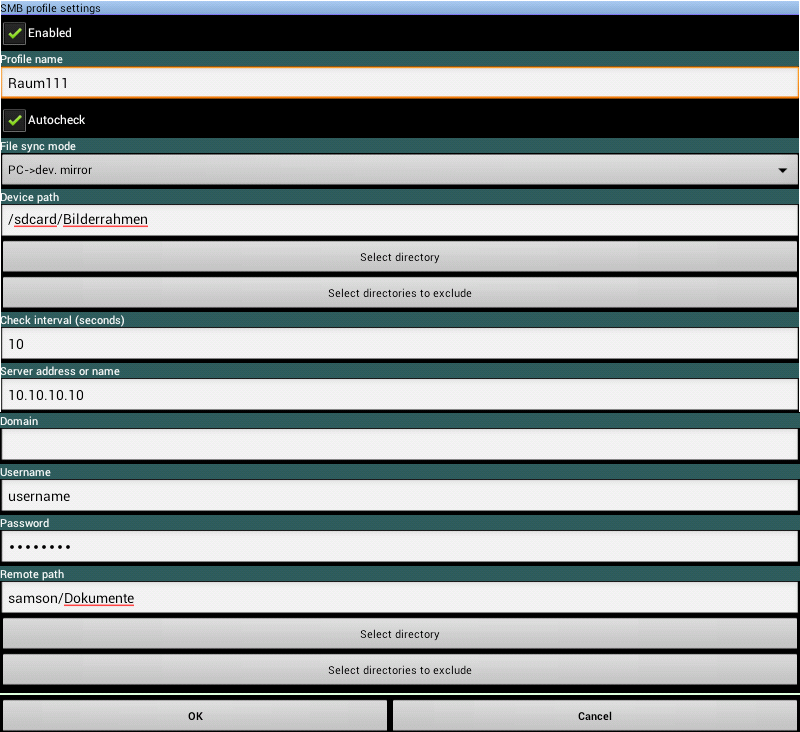
\includegraphics[width=.7\textwidth]{pcfilsync_conf.png}\\ % PNG-File
      \end{figure}
      Nun ist die App fertig konfiguriert und der Synchronisation-Service sollte schon automatisch gestartet sein.
      Ab dem zweiten Mal, muss die PcFileSync-App nur noch einmal gestartet werden, damit der Service startet, die Konfiguration bleibt erhalten.    
  \subsection{Konfigurieren der Applikation - PhotoFrameApp}
  	Die PhotoFrame-Applikation dient dazu, dass die Bilder aus dem synchronisierten Verzeichnis mittels einer Diashow ausgegeben werden.
    \begin{itemize}
      \item Starten sie die App mittels der Schaltfläche ``Start/configure PhotoFrameApp!''.
      \item Am oberen Rand sehen sie dann in der App eine Schaltfläche mit einem kleinen Zahnrad, klicken sie dort drauf, um in die Einstellungen zu gelangen.
      \item Angelangt im Einstellungs-Dialog, legt man zuerst das Intervall zwischen den Bildern fest. Zum Beispiel ein Intervall von 20 Sekunden.
      \item Als nächstes legt man die Art der Reihenfolge der Diashow fest. Im Fall eines Türschilds, würden wir die Reihenfolge nach Datum epmfehlen.
      \item Daraufhin muss das erneute einlesen des Ordners aktiviert werdenm, dazu machen sie bitte einen Haken bei ``Erneutes Laden einschalten''. Darunter legen sie das Intervall fest, wie oft der Ordner neu eingelesen wird. Wir würden ein Intervall von 30 Sekunden vorschlagen, das sollte ausreichend oft sein.
      \item Darauffolgend kann man eine Option aktivieren, die es veranlasst, dass nach dem ersten mal starten einer Diashow, die App bei nächsten Start wieder die Diashow im selben Ordner startet. Diese Option empfehlen wir ebenfalls, man aktiviert sie mit einem Haken bei Punkt ``Nach dem Neustart automatisch Fotos anzeigen.''.
      \item Nun folgen noch ein paar Anzeigeoptionen für die Diashow, diese sind natürlich nur eine Empfehlung. Sie beeinträchtigen also nicht die Funktion des Tablets als intelligentes Türschild.
      \begin{itemize}
        \item Als erstes kann man das Standardlayout zur Anzeige der Bilder auswählen. Wir würden hier das Layout ``Vollbild Fotos'' empfehlen
        \item Danach kommt der Punkt ``Deckkraft starten'', hier kann man einstellen, ob die Bilder nachdem erscheinen langsam heller werden. Diese Option ist nach unserer Meinung, bei einem Türschild nicht sehr sinnvoll, also würden wir empfehlen diesen auf dem Wert ``255'' zu belassen.
        \item Als nächstes kann man aktivieren bzw. deaktivieren ob in der Diashow eine Foto Nummerierung zusahen sein soll. Wir würde die Option deaktivieren, ist bei einem Türschild nicht relevant.
        \item Daraufhin kann man auswählen ob der Dateiname angezeigt werden soll, was wir ebenfalls nicht empfehlen würden.
        \item Zum Schluss kommen die beiden Optionen ``Zeige Vollbild'', die Bilder werden also möglichst groß skaliert in Abhängigkeit der Auflösung des Bildschirms und ``Werden im Querformat.'', also alle Bilder werden ins Querformat gebracht. Diese beiden Optionen würden wir aktivieren.
      \end{itemize}
    \end{itemize}
    Damit ist die Konfiguration der PhotoframeApp weitestgehend abgeschlossen, beim endgültigen starten der Applikation, nach der Einrichtung des Standby-Service, muss man dann nur noch den entsprechenden Ordner, der mittels PcFileSync synchronisiert ist, auswählen.
  \subsection{Standby-Service konfigurieren}
    Der Standby-Service wurde dazu entwickelt, das Tablet zu bestimmten Zeiten aus dem Standby aufzuwecken bzw. in den Standbymodus zu versetzen.
    \begin{itemize}
      \item In der rechten Spalte der IDC-App haben wir zwei TimePicker zum festlegen der Wake-UP- und Sleep-Time. Diese legt man nun nach seinen Wünschen fest.
      \item Danach können sie über den Button ``Start Standby \& NoTouch Service'' den Service starten.
      \item Vor dem Start wird auch in der Applikation noch mal der Hinweis gegeben, dass sie noch ca. 5 Minuten haben bis der Touchscreen gesperrt wird. Danach ist das Tablet nur noch durch einen Neustart wieder normal zu verwenden.
    \end{itemize}
    In der verbleibenden Zeitspanne, muss nun endgültig die PhotoFrameApp gestartet und die Diashow ausgeführt werden. Daraufhin ist das Tablet nun so konfiguriert, das es sich mit dem gewählten Verzeichnis synchronisiert, es eine Diashow mit dessen Inhalt ausgibt, es nicht von Unbefugten benutzt werden kann und es sich zu bestimmten Zeiten in den Standbymodus versetzt und daraus auch wieder erwacht.
\end{flushleft}
